\documentclass[11pt]{article}

% Page Setup
\usepackage{geometry}
\geometry{
    a4paper,
    margin={2.5cm}
}

% Basic Packages
\usepackage{amssymb}
\usepackage{stmaryrd}
\usepackage{amsmath}
\usepackage{amsthm}
\usepackage{mathtools}
\usepackage{mathpartir}
\usepackage{enumitem}
\usepackage{mathabx}

% Font
\usepackage{charter}

% Bibliography and index
\usepackage[backend=biber, style=numeric]{biblatex}
\addbibresource{refs.bib}
\usepackage{makeidx}
\makeindex

% Colors and Graphics
\usepackage[dvipsnames, x11names]{xcolor}
\usepackage{tikz}
\usetikzlibrary{
    cd,
    fit,
    calc,
    positioning,
    arrows,
    automata,
    shapes
}
\tikzset{
    baseline = (current bounding box.center),
    every state/.append style = {
        rectangle,
        rounded corners=5pt,
		inner sep = 3pt,
		minimum size = 18pt,
		initial text = {},
        fill=Azure1
	},
	every edge/.append style = {
		->,
		>=stealth,
		bend angle=10,
		thick
	}
}
\usepackage{musicography}
\usepackage{graphics}
\graphicspath{../imgs/}

% Hyperlinks
\usepackage{hyperref}
\hypersetup{
    colorlinks,
    linkcolor   = black,
    filecolor   = RubineRed,
    urlcolor    = RubineRed,
    citecolor   = RubineRed,
    pdftitle    = {Notes on Behavioural PDEs}
}
\usepackage[capitalize]{cleveref}

% Environments
\theoremstyle{theorem} % In Italics
\newtheorem{theorem}                    {{\color{Purple}Theorem}}[section]
\newtheorem{lemma}          [theorem]   {{\color{Magenta}Lemma}}
\newtheorem{proposition}    [theorem]   {Proposition}
\newtheorem{corollary}      [theorem]   {Corollary}
\newtheorem{question}                   {{\color{red}Question}}

\theoremstyle{definition} % Not in italics
\newtheorem{definition}     [theorem]   {{\color{NavyBlue}Definition}}
\newtheorem{example}        [theorem]   {{\color{ForestGreen}Example}}
\newtheorem{problem}                    {{\color{BurntOrange}Problem}}

\theoremstyle{remark} % Subdued label
\newtheorem{remark}[theorem]        {{\color{Gray}Remark}}

% (1), (2), ...
\renewcommand\labelenumi{(\theenumi)}

% Go nuts with line breaks 
\allowdisplaybreaks

%%%%%%%%%%
% MACROS %
%%%%%%%%%%

% Categories and functors
\newcommand{\Set}{\mathbf{Set}}
\newcommand{\Alg}{\mathbf{Alg}}
\newcommand{\Coalg}{\mathbf{Coalg}}
\newcommand{\Cat}{\mathbf{C}}
\newcommand{\Id}{\mathrm{Id}}
\newcommand{\op}{\mathrm{op}}
\newcommand{\obj}{\mathrm{obj}}
\newcommand{\Std}{\mathsf{S}}

% Natural Transformations
\newcommand{\id}[1]{\mathsf{id}_{#1}}
\newcommand{\unit}[1]{\eta_{#1}}
\newcommand{\mult}[1]{\mu_{#1}}
\newcommand{\incl}{\mathsf{incl}}
\newcommand{\proj}{\mathsf{proj}}

% Algebras and Monads
\newcommand{\T}{\mathsf{T}}
\newcommand{\Pow}{\mathcal{P}}
\newcommand{\Dis}{\mathcal{D}}
\newcommand{\FF}{\mathcal F}

% Numbers and Standard notation
\newcommand{\NN}{\mathbb{N}}
\newcommand{\ZZ}{\mathbb{Z}}
\newcommand{\RR}{\mathbb{R}}
\newcommand{\QQ}{\mathbb{Q}}
\newcommand{\pRR}{\mathbb{R}_{+}}

\newcommand{\dom}{\mathrm{dom}}
\newcommand{\cod}{\mathrm{cod}}

\newcommand{\dd}{\mathsf{d}}
\newcommand{\der}{\mathbf{\partial}}
\newcommand{\eval}{\mathsf{eval}}
\newcommand{\head}{\mathsf{head}}
\newcommand{\beh}{\mathsf{beh}}

\newcommand{\Grph}{\operatorname{Grph}}

\newcommand{\Grid}{\mathsf{Grid}}

\newcommand{\pulse}{\mathsf{e}}
\newcommand{\switch}{\mathsf{s}}

\newcommand{\inv}{{-1}}

% Semantics
\newcommand{\sem}[1]{\llbracket{#1}\rrbracket}
\newcommand{\bigsem}[1]{\Big\llbracket{#1}\Big\rrbracket}
\newcommand{\e}{\varepsilon}

\newcommand{\wordCat}[1]{\{\hspace*{-2.5pt}| #1 |\hspace*{-2.5pt}\}^*}

% Transitions
\newcommand{\tr}[1]{
    \mathrel{
        \raisebox{-1pt}{
            \(\xrightarrow{#1}\)
        }
    }
}
\newcommand{\bisim}{\mathrel{\raisebox{1pt}{\(\underline{\leftrightarrow}\)}}}

% Text
\newcommand{\code}[1]{\texttt{#1}}
\newcommand{\codeblock}[1]{
    \begin{center}
        \parbox{0.8\textwidth}{
            \ttfamily
            #1
        }
    \end{center}
}

% Boolean statements
\newcommand{\OR}{~\mathrm{or}~}
\newcommand{\AND}{~\mathrm{and}~}
\newcommand{\NOT}{\mathrm{not}~}
\newcommand{\IMPLIES}{~\mathrm{implies}~}
\newcommand{\FORALL}{\mathrm{for\ all}~}
\newcommand{\EXISTS}{\mathrm{there\ exists}~}
\newcommand{\SUCHTHAT}{~\mathrm{such\ that}~}








% Title
\title{CSCI 341 Problem Set 1}
\author{Games and State Machines; Automata}
\date{Due
    Monday, September 1
}

\begin{document}

\maketitle

\subsection*{Games and State Machines}

\begin{problem}
    [Always an Upper Bound]
    Let \(M = (G, L, S, E, A, C)\) be a directional maze with the set of legal moves \(A = \{\Uparrow, \Rightarrow\}\).
    Prove that \(\mathcal S(M)\) is finite (there are only finitely many elements) by calculating an upper bound on the number of all possible legal paths through an \(n\times m\) directional maze.
\end{problem}

\begin{problem}
    [Reverse Engineering]
    Find a Sokoban game that represents state \(s_1\) in abstract state diagram (A).
    Replace the states in the state diagram with drawings of each state of the Sokoban game.

    \begin{figure}[h]
        \centering
        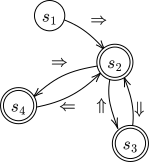
\includegraphics{../imgs/reverseengineering.png}
        \caption{Abstract state diagram (A).}
    \end{figure}
\end{problem}

\begin{problem}
    [Impossibility]
    Prove that there \emph{does not} exist a directional maze that represents state \(s_1\) in abstract state diagram (A).
\end{problem}

\subsection*{Reading Words}

\begin{problem}
    [Repeated Derivatives]
    Let \(\mathcal A = (Q, A, \delta, F)\) be an automaton, let \(x \in Q\), and \(w \in A^*\) and \(a \in A\).
    Prove the following identity:
    \[
        \delta(x, w a) = \{z \mid z \in \delta(y, a) \text{ for some } y \in \delta(x, w)\}
    \]
\end{problem}

\begin{problem}
    [Determinstic Extension]
    Let \(\mathcal A = (Q, A, \delta, F)\) be a total deterministic automaton.
    Let \(x \in Q\) and \(w \in A^*\).
    Prove that \(\delta(x, w)\) has exactly one element using Induction on Words.
\end{problem}

\subsection*{Language Acceptance}

\begin{problem}
    [Let 'em Cook]
    For each of the following languages \(L_i \subseteq A^*\) below, design an automaton \(\mathcal A_i = (Q_i, A, \delta_i, F_i)\) with a state \(x \in Q_i\) such that \(x\) accepts \(L_i\), and briefly explain why your automaton accepts \(L_i\).
    Note that \(A = \{a, b\}\) in all of the cases below.
    \begin{enumerate}
        \item \(L_1 = \{a, aa, aaa\}\)
        \item \(L_2 = \{w \in A^* \mid \text{\(w\) ends with \(b\)}\}\)
        \item \(L_3 = \{w \in A^* \mid \text{\(w\) has an even number of \(a\)'s}\}\)
        \item \(L_4 = \{w \in A^* \mid \text{\(w\) has \(3k+1\) many \(a\)'s for some \(k \ge 0\)}\}\)
        \item \(L_5 = \{w \in A^* \mid \text{\(w\) either has \(3k+1\) or \(3k + 2\) many \(a\)'s for some \(k \ge 0\)}\}\)
        \item \(L_6 = A^* \setminus L_2\)
    \end{enumerate}
\end{problem}

\begin{problem}
    [Pythonic Automaton]
    Write a Python script in the same format as the Pythonic Automaton I that implements state \(s_1\) in abstract state diagram (A) from the games and puzzles section. 
    Submit your program as a .py file in the programming submission box (see the other Gradescope assignment).
\end{problem}

\subsection*{Finite and Infinite Automata}

\begin{problem}
    [Unravelling an Infinite Language]
    Draw a state diagram of all of the languages that are reachable from the language \(L = \{(ab)^n \mid n \in \mathbb N\}\) in the Brzozowski automaton by taking \(a\)- and \(b\)-derivatives (the words in this language are \(\varepsilon\), \(ab\), \(abab\), ...). 
    Include all of the double-circled states to indicate which languages are accepting states of the Brzozowski automaton.
    What language is accepted by \(L\)?
\end{problem}

\begin{problem}
    [Language Accepts Itself]
    Let \(L \subseteq A^*\) be any language. 
    Prove that \(\mathcal L(\mathcal A_{Brz}, L) \subseteq L\).
\end{problem}

\end{document}